\section{Exercise five}

Let's calculate the mean time to failure (MTTF) of a RAID 10 and RAID 01 setup with the following specifications:
\begin{itemize}
    \item $N=8$ disks.
    \item Mean Time to Repair (MTTR) of four days.
    \item Mean Time to Failure (MTTF) of a single disk is 2200 days.
\end{itemize}
Compte the Mean Time to Failure (MTTF) in case of:
\begin{enumerate}
    \item RAID 10. 
    \item RAID 01. 
\end{enumerate}

\subsection*{Solution}
\begin{enumerate}
    \item For the RAID 10 setup:
        \begin{figure}[H]
            \centering
            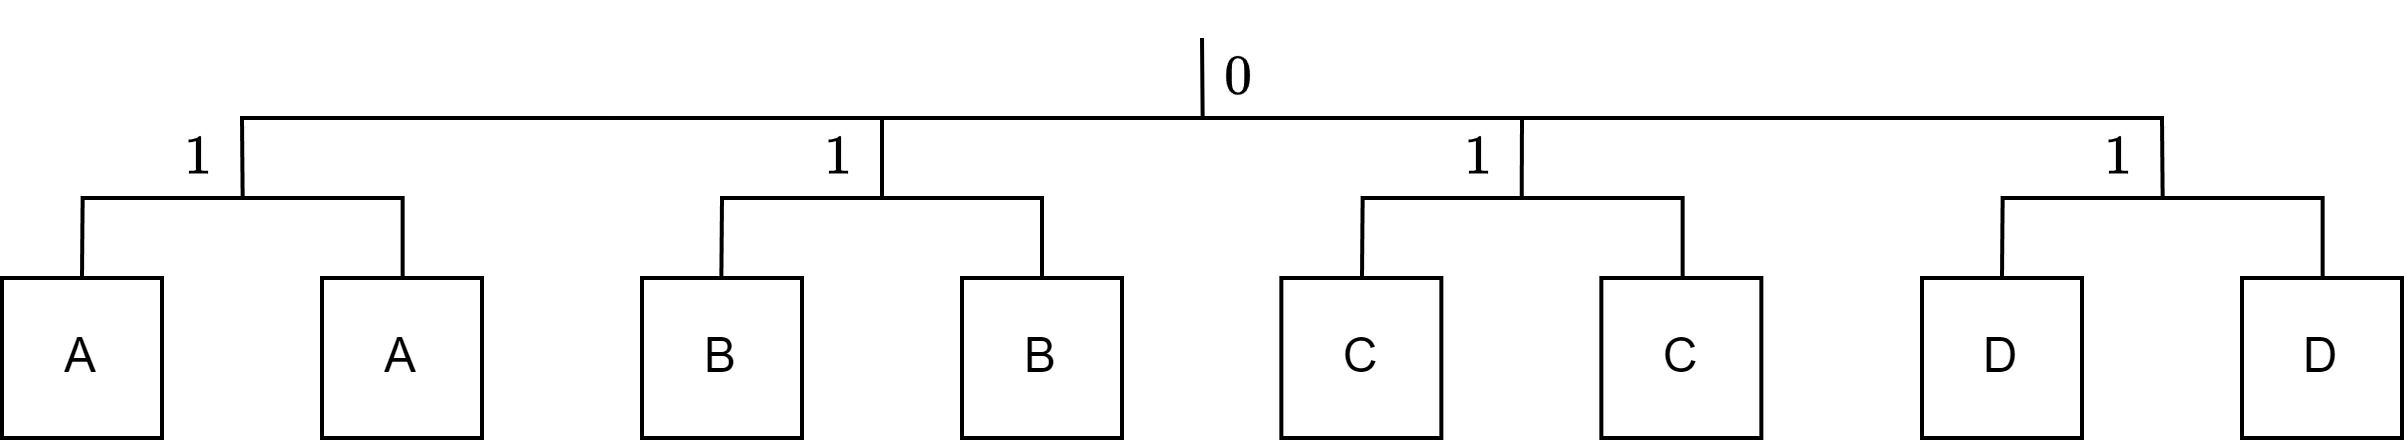
\includegraphics[width=0.75\linewidth]{images/510.png}
        \end{figure}
        The failure rate is:
        \[\lambda_{\text{RAID 01}}=\dfrac{N}{\text{MTTF}}\left(\dfrac{1}{\text{MTTF}}\text{MTTR}\right)=\dfrac{8\cdot\text{MTTR}}{\text{MTTF}^2}\]
        Hence, the mean time to failure is:
        \[\text{MTTF}_{\text{RAID 10}}=\dfrac{1}{\lambda_{\text{RAID 10}}}=\dfrac{\text{MTTF}^2}{8\cdot\text{MTTR}}=\dfrac{2200^2}{8\cdot 4}\]
    \item For the RAID 01 setup:
        \begin{figure}[H]
            \centering
            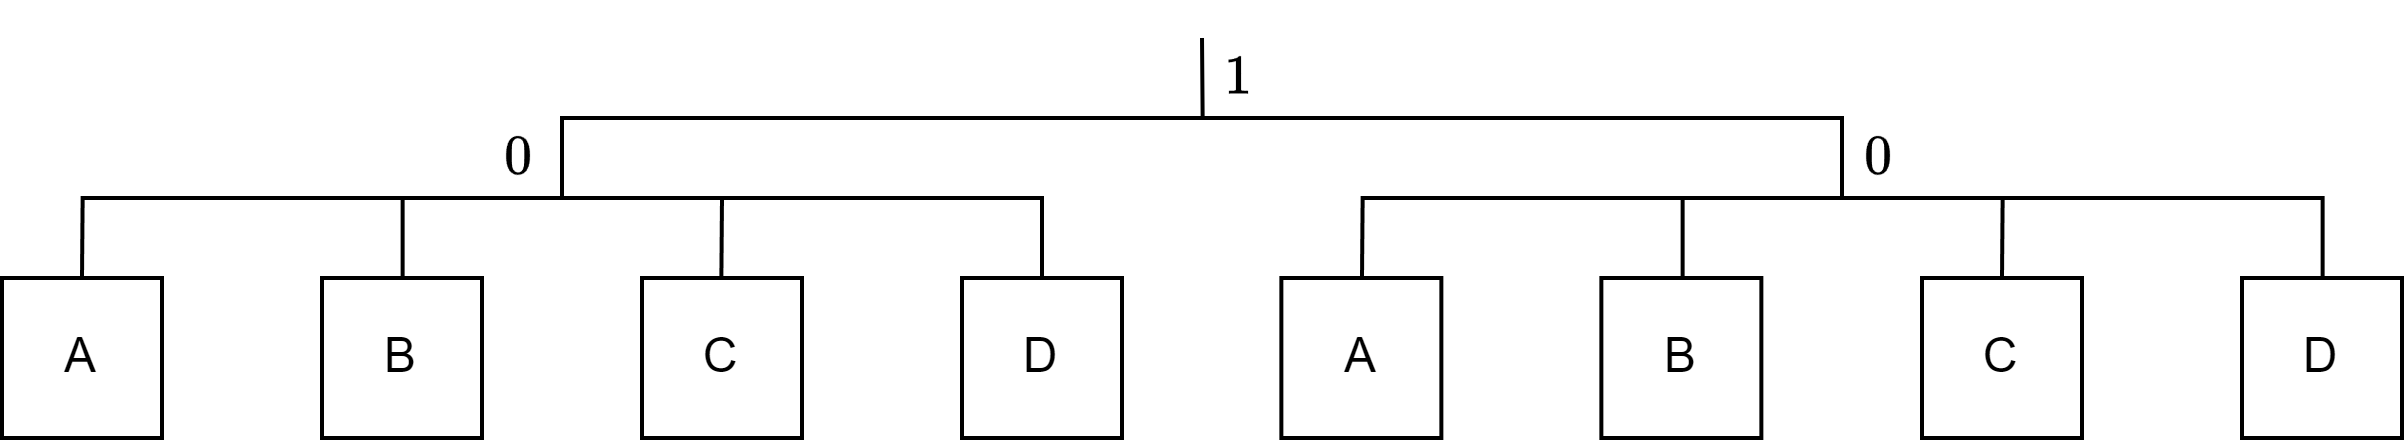
\includegraphics[width=0.75\linewidth]{images/501.png}
        \end{figure}
        The failure rate is:
        \[\lambda_{\text{RAID 01}}=\dfrac{N}{\text{MTTF}}\left(\dfrac{\frac{N}{2}}{\text{MTTF}}\text{MTTR}\right)=\dfrac{32\cdot\text{MTTR}}{\text{MTTF}^2}\]
        Thus, the mean time to failure is:
        \[\text{MTTF}_{\text{RAID 01}}=\dfrac{1}{\lambda_{\text{RAID 10}}}=\dfrac{\text{MTTF}^2}{32\cdot\text{MTTR}}=\dfrac{2200^2}{32\cdot 4}\]
\end{enumerate}